\section{Реализация}
    Задача автоматического установления связей между твитами и новостями решается посредством написания программного комплекса,
    который обладает следующими возможностями:
    \begin{enumerate}
        \item сбор необходимой для решения задачи информации;
        \item построение наборов данных;
        \item применение к наборам данных методов машинного обучения;
        \item получение рекомендаций новостей для произвольных твитов;
        \item вариативность в выборе метода для построения рекомендаций;
        \item возможность получить информацию о качестве используемого метода.
    \end{enumerate}

    Программный комплекс реализуется с использование языка программирования Python 2.7.

    \subsection{Архитектура}
    Программный комплекс позволяет производить все требуемые для решения задачи преобразования над данными, а именно:
    \begin{enumerate}
        \item получение данных из твиттера;
        \item получение данных из новостной rss-ленты;
        \item расшифровка сокращённых URL;
        \item автоматическое построение набора данных;
        \item построение моделей для методов WTMF и WTMF-G;
        \item построение рекомендаций на основе методов WTMF, WTMF-G и TF-IDF;
        \item оценка качества рекомендаций;
        \item получение результатов рекомендаций в пригодном для чтения формате;
    \end{enumerate}
%    Результаты всех преобразований, за исключением оценки качества и получения рекомендаций, хранятся в специальном промежуточном
%    хранилище~(побробное описания хранилища производится в разделе~\ref{sec:documentation}).

    Каждое преобразование, в общем случае, независимо от других.
    Для построения рекомендаций, необходимо выполнить цепочку преобразований.
    Примеры цепочек преобразований для получения данных, построения рекомендаций и оценки их качества приводятся ниже.
    
    Визуализация цепочек преобразований производится при помощи рисунков, использующих элементы блок-схем~\cite{flowchart_gost}.
    Для удобства восприятия блоки действия~(изображаются прямоугольником) выделяются зелёным цветом, 
    а прочие используемые блоки, такие как ввод-вывод данных~(изображаются параллелограммом) и хранимые 
    данные~(изображаются фигурой, представляющей собой прямоугольник, в котором две противолежащие стороны 
    заменены на две одинаковые и параллельные кривые, совпадающие с секцией окружности), выделяются синим цветом.
    
    Получение данных заключается в скачивании новостей из RSS потоков и твитов, с использованием Twitter Streaming API, в течение длительного промежутка времени, с последующим помещением всех данных в промежуточное хранилище. В работе в качестве хранилища выступает python shelve.
    Получение данных в виде блок-схемы изображен на рисунке~\ref{pic:consumer_flowchart}.
    \begin{figure}[h!]
            \center
            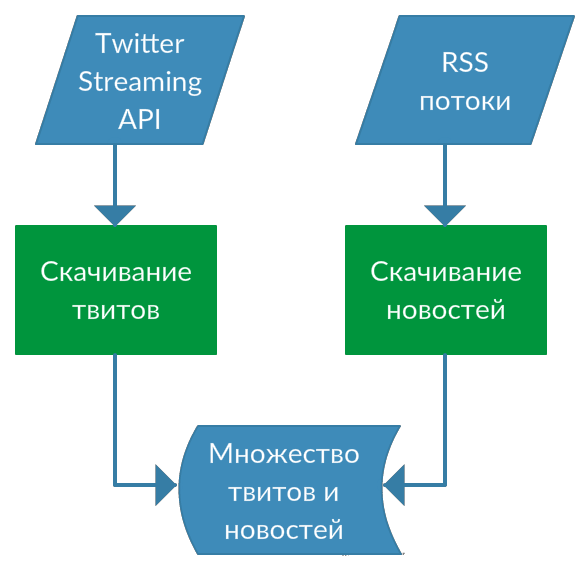
\includegraphics[scale=0.4]{twnews_consumer_flowchart.png}
            \caption{Блок-схема получения данных}
            \label{pic:consumer_flowchart}
    \end{figure}

    На основе полученного множества новостей и твитов происходит автоматическое построение набора данных. В рамках автоматического построения набора данных происходит расшифрка сокращённых URL.
    Набор данных эта структура состоящая из списка новостей и списка твитов, где для каждого твита указана ссылка на единственную новость.

    Результатом работы всех реализованных методов является сопоставление численных векторов~(векторов для сравнения) каждому обрабатываемому тексту, с помощью которых можно оценить насколько похожи любые два текста. 

    Метод TF-IDF не имеет стадии обучения модели, поэтому применяется непосредственно к набору данных и получает вектора для сравнения, для всех текстов, которые были переданы ему на вход.
    Получаемые векторы обладают размерностью совпадающей с размером корпуса.

    В отличие от метода TF-IDF методы WTMF и WTMF-G состоят из двух стадий: обучения и применения модели. На стадии обучения методы строят модель~(в сериализованной модели помимо самой модели содержится набор данных, на основе которого была построена модель) и получают вектора для сравнения для всех элементов набора данных. На стадии применения методы WTMF и WTMF-G на основе ранее построенной модели для произвольного множества твитов строят векторы для сравнения полученных на вход твитов и новостей из набора данных.

    На основе множества, состоящего из твитов и новостей, для каждого элемента в котором существует вектор для сравнения, строятся рекомендации.
    Рекомендации представляют собой множество твитов, к каждому из которых сопоставлен ранжированный по мере убывания схожести список новостей.

    \begin{figure}[h!]
            \center
            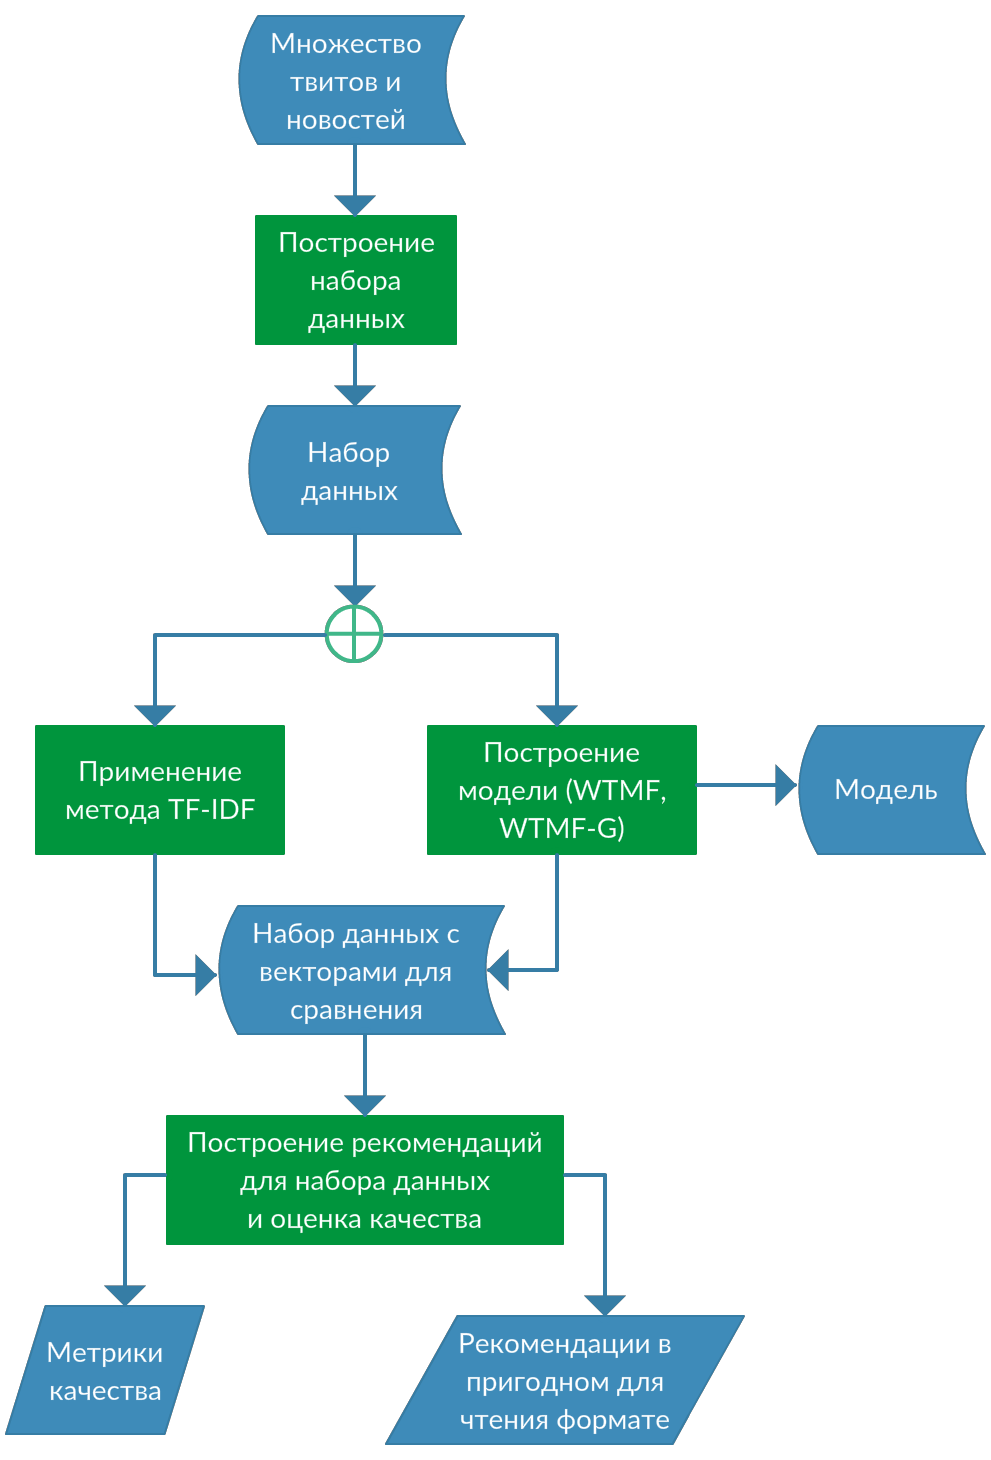
\includegraphics[scale=0.32]{twnews_flowchart_1.png}
            \caption{Блок-схема процесса оценки качества используемых методов}
            \label{pic:twnews_flowchart_1}
    \end{figure}

    На основе построенных рекомендаций можно как произвести оценку качества ранее использованного метода, так и получить их в виде текстового файла,
    который содержит информацию в пригодном для чтения формате.
    Оценка качества использованного метода производится при условии построения рекомендаций для набора данных.
    Процесс оценки качества различных методов рекомендаций, а также получение рекомендаций для твитов из набора данных изображён на рисунке~\ref{pic:twnews_flowchart_1}.

    Дополнительным результатом изображённого на рисунке~\ref{pic:twnews_flowchart_1} процесса является построенная модель (для методов WTMF и WTMF-G), которую можно применить на произвольное множество твитов. Процесс получения рекомендаций для произвольных твитов изображён на рисунке~~\ref{pic:twnews_flowchart_2}.
    
    \begin{figure}[h!]
            \center
            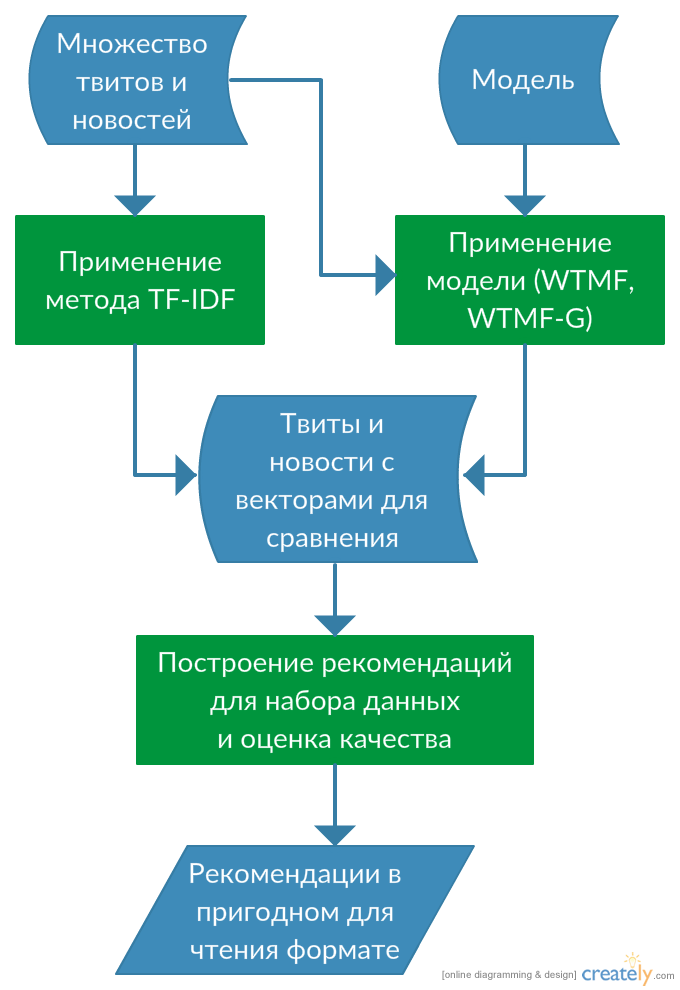
\includegraphics[scale=0.32]{twnews_flowchart_2.png}
            \caption{Блок-схема процесса получения рекомендаций для различных методов}
            \label{pic:twnews_flowchart_2}
    \end{figure}

    %\textcolor{red}{заключительный абзац}

    




    \subsection{Получение данных}
    Для получения данных~(твитов и новостей) необходимо:
    \begin{enumerate}
        \item реализовать скачивание твитов и новостей из разных новостных источников;
        \item определить формат хранения скачиваемых данных;
        \item скачать твиты за определённый промежуток времени;
        \item расшифровать сокращённые URL;
        \item определить список наиболее популярных новостных источников в твиттере;
        \item в течение длительного времени собрать данные как с твиттера, так и с новостных источников.
    \end{enumerate}

    \subsubsection{Cкачивание твитов}
        Для скачивания данных твиттера используется Twitter Streaming API~---~сервис,
        предоставляющий разработчикам возможность в реальном времени получить поток данных твиттера~\cite{twitter_streaming}.
        С помощью Twitter Streaming API можно бесплатно получить 1\% от всех публичной информации твиттера: публикация и удаления твитов.

        Для работы с Twitter Streaming API необходимо на сайте~https://apps.twitter.com/ зарегистрировать новое приложение и получить набор секретных ключей,
        которые требуются для авторизации.
        Для упрощения работы с Twitter Streaming API используется библиотека tweepy~\cite{tweepy}, предоставляющая удобный интерфейс на языке Python.

        Twitter Streaming API предоставляет данные в формате JSON~(от англ. JavaScript Object Notation)~---~текстовый формат обмена данными, удобный для чтения человек,
        первоначально создавался как формат на текстового описания и сериализации объектов языка программирования JavaScript.

        В рамках работы используется информация публикации твитов.
        Каждое событие о создании твита описывается в виде большого количества параметров~(несколько десятков), в работе используются следующие:
        \begin{enumerate}
            \item created\_at~---~дата создания,
            \item id~---~уникальный идентификатор,
            \item retweeted\_status~---~существует, только если твит является ретвитом, содержит информацию о ретвитнутом твите,
            \item lang~---~язык,
            \item entities~---~информация о хэштегах и ссылках, которые упоминаются  в твите,
            \item text~---~текст твита.
        \end{enumerate}

        Каждое событие о создании твита обрабатывается.
        Результатом обработки является структура данных, в которой содержится вся необходимая информация о созданном твите.
        Обработка происходит следующим образом:
        \begin{enumerate}
            \item Если твит не на русском языке, он отбрасывается.
            \item Если твит является ретвитом, то взводится специальный флажок и дальнейшая работа происходит с исходным ретвитнутым твитом.
            Это делается для того, чтобы получить полноценный текст исходного твита.
            \item Из поля entities извлекается информация о хэштегах и ссылках, встречаемых в твите.
        \end{enumerate}
        Вся полученная информация помещается в хранилище твитов. Хранилище твитов реализованно использованием библиотеки python shelve~\ref{shelve}.

    \subsubsection{Скачивание новостных статей}
        Новостные статьи скачиваются в формате
        \textit{RSS}~---~ семейство XML-форматов, предназначенных для описания лент новостей, анонсов статей, изменений в блогах и т.п.
        Формат RSS выбран ввиду его поддержки всеми популярными новостными источниками.
        Для работы с потоками RSS используется библиотека feedparser~\cite{feedparser}, позволяющая скачивать и анализировать данные в формате RSS.

        RSS поток представляет собой переодически обновляемый список статей. Каждая статья обладает рядом параметров в работе используются следующие:
        \begin{enumerate}
            \item published~---~дата создания,
            \item summary~---~краткое изложение новостной статьи,
            \item link~---~URL, который ведёт на описываемую новостную стать.,
            \item title~---~заголовок новостной статьи,
        \end{enumerate}

        Скачивание RSS-потоков происходит следующим образом: переодически получается актуальное состояние всех RSS потоков, из них вычленяются все новые статьи,
        которые предобрабатываются и добавляются в хранилище новостей. Хранилище новостей реализованно с использованием библиотеки python shelve~\ref{shelve}.

    \subsubsection{Расшифровка сокращённых URL}
        \textit{Сокращение URL}~---~это сервис, предоставляемый разными компаниями, заключающийся в создании дополнительного, в общем случае более короткого URL, введущего на искомый адрес.
        Обычно применяется с целью экономии длины сообщения или для предотвращения непреднамеренно искажения URL.
        В общем случае механизм сокращений реализовывается путём переадресации короткого URL на искомый.

        В твиттере все ссылки автоматически сокращается с помощью сервиса \textit{t.co}. Также многие ссылки добавляются в твиттер уже сокращёнными через сторонние сервисы.
        Для автоматического выявления связей между твитами и новостями с целью построения тестового набора данных необходимо уметь по сокращённому URL получить исходный.

        \textit{Расшифровка сокращённых URL}~---~процесс получения по сокращённому URL исходного адреса.
        На практике часто встречается применение сокращения URL каскадом: сокращение уже сокращённого URL,
        в таком случае расшифровка заключается в получении исходного URL, который не является сокращённой ссылкой.
        Можно трактовать задачу расшифровки следующим образом: необходимо получить URL адрес на котором завершится процесс переадресации.

        Расматриваемая задача требует обработки большого количества твитов и следовательно большого количества расшифровок сокращённых URL~(
        в главе~\ref{sec:impl_dataset} получено, что количество ссылок, требуемых для анализа превышает $10^5$).
        Поэтому возникает требование к повышенной эффективности решения.

        В качестве базового решения используется стандартный API языка Python, позволяющий получить содержимое веб-страницы по URL,
        а следовательно адрес целевой страницы на которую вела сокращённая ссылка. Случаи в которых исходный URL не был получен, будем называть ошибочными.
        Базовое решение было оптимизировано следующим образом:
        \begin{enumerate}
            \item Работа только с заголовками ответа. Это позволило снизить количество данных пересылаемых по сети.
            Работа с заголовками требует логики для принятия решения об остановке~---~то есть выявления искомого URL.
            %\item Работа лишь с заголовками ведёт к большому количеству ошибок, для преодоления этого используется следующая логика:
%             если на основе заголовков не удалось правильно определить целевой URL, то запускается базовое решение.
            \item Использование многопоточности.
            Так как большую часть времени код, получающий заголовок страницы ждёт ответа сервера, то асинхронность позволит значительно увеличить быстродействие.
            \item Использование <<воронки>> данных. При увеличении количества потоков стало появляться большее количество ошибок,
            ввиду того, что загруженность интернет-канала повышает время ответа http-запросов.
            Для их снижения было выбран подход <<воронки>> данных с последующей коррекцией ошибок. Данный подход на первом этапе обрабатывает все ссылки в $N$ потоков,
            на втором этапе все ошибочные ссылки полученные на первом обрабатываются в $\dfrac{N}{10}$ потоков и так далее, вплоть до 1 потока на итерацию.
        \end{enumerate}
%
%site_open_unshorter 2.7021s; 0.00%
%header_unshoter 2.3535s; 0.00%
%unshorten_url 1.4018s; 0.00%
%^[[A^[[Aweb_unshoter 1.8972s; 0.00%

%
%
%        Замеры времени работы в рамках оптимизации приведены в таблице~\ref{tabular:unshort}.
%
%        \begin{table}[ht!]
%            %\small
%            \caption{Оптимизация расшифровки сокращённых URL\bigskip}
%            \centering
%
%            \label{tabular:unshort}
%            \begin{tabular}{|p{5cm}|c|c|c|}
%                \hline
%                \bf{\specialcell{Добавленная \\ оптимизация}} &
%                \bf{\specialcell{Время на \\ расшифровку \\ 1000 URL}} &
%                \bf{\specialcell{Прирост \\ производительности \\ (\%) }} &
%                \bf{\specialcell{Относительное \\ число ошибок \\ (\%) }} \\ \hline
%
%                Базовое решение & 123 & 123 & 123 \\ \hline
%                Работа только с заголовками ответа & 123 & 123 & 123 \\ \hline
%                Использование многопоточности & 123 & 123 & 123 \\ \hline
%                Использование <<воронки>> данных & 123 & 123 & 123 \\ \hline
%            \end{tabular}
%        \end{table}
%        На основании таблицы ... видно ...
%
%        Также для обоснования необходимости самостоятельной реализации подобного алгоритма в таблице приводится сравнение с популярным сервисом \
%        для расшифровки ссылок \url{unshorten.it}~(работа с сервисом производилась через публичный API).

    \subsubsection{Выявление источников новостей}
        Задача выявления источников новостей требует статистического исследования ссылок, которые встречаются в твитах.
        Для определения ссылок ведущих на новостные источники из всех URL извлекалось полное доменное имя~(в дальнейшем доменное имя).
        Также стоит отметить, что новостные агрегаторы~(к примеру Яндекс-новости, Рамблер-новости) не рассматривались ввиду того, что они агрегируют
        очень большое количество новостных статей с множества разнородных источников. То есть очень сложно собрать и в дальнейшем обрабатывать эталонный набор новостей.

        Для грубой оценки использовалась выборка 1, содержащая 35704 твитов, 13670 ссылок, 12510 уникальных ссылок.
        Статистика по 20 наиболее часто встречаемым доменным именам в выборке 1 представленна в таблице~\ref{tabular:domain_1}.
        \begin{table}[ht!]
            %\small
            \caption{20 наиболее часто вречаемых доменных имён в выборке 1 (всего 12510 уникальных ссылок)\bigskip}
            \centering

            \label{tabular:domain_1}
            \begin{tabular}{|c|c|c|c|}
                \hline
                \bf{\specialcell{Доменное имя}} &
                \bf{\specialcell{Количество \\ ссылок}} &
                \bf{\specialcell{Процент от \\ общего числа\\ ссылок}} &
                \bf{\specialcell{Новостной источник}} \\ \hline
                twitter.com & 3521 & 25.76 & нет \\ \hline
                www.facebook.com & 1418 & 10.37 & нет \\ \hline
                t.co & 405 & 2.96 & нет \\ \hline
                www.youtube.com & 315 & 2.30 & нет \\ \hline
                news.yandex.ru & 239 & 1.75 & нет \\ \hline
                su.epeak.in & 214 & 1.57 & нет \\ \hline
                www.instagram.com & 198 & 1.45 & нет \\ \hline
                www.periscope.tv & 191 & 1.40 & нет \\ \hline
                l.ask.fm & 121 & 0.89 & нет \\ \hline
                lifenews.ru & 109 & 0.80 & да \\ \hline
                ria.ru & 108 & 0.79 & да \\ \hline
                vk.com & 93 & 0.68 & нет \\ \hline
                news.7crime.com & 82 & 0.60 & нет \\ \hline
                lenta.ru & 74 & 0.54 & да \\ \hline
                russian.rt.com & 61 & 0.45 & да \\ \hline
                linkis.com & 57 & 0.42 & нет \\ \hline
                www.gazeta.ru & 53 & 0.39 & да \\ \hline
                tass.ru & 43 & 0.31 & да \\ \hline
                www.swarmapp.com & 42 & 0.31 & нет \\ \hline
                pi2.17bullets.com & 36 & 0.26 & нет \\ \hline
            \end{tabular}
        \end{table}

        Как видно из таблицы~\ref{tabular:domain_1} популярные новостные агенства составляют лишь малую долю от общего количества используемых ссылок (3.3\%).
        Для получения более точной количественной информации за неделю собрана выборка 2, содержащая 341863 твитов, 134945 ссылок, 115940 уникальных ссылок.
        Статистика по 20 наиболее часто используемым доменным именам в выборке 2 представленна в таблице~\ref{tabular:domain_2}.
        \begin{table}[ht!]
            %\small
            \caption{20 наиболее часто вречаемых доменных имён в выборке 2 (всего 115940 уникальных ссылок)\bigskip}
            \centering

            \label{tabular:domain_2}
            \begin{tabular}{|c|c|c|c|}
                \hline
                \bf{\specialcell{Доменное имя}} &
                \bf{\specialcell{Количество \\ ссылок}} &
                \bf{\specialcell{Процент от \\ общего числа\\ ссылок}} &
                \bf{\specialcell{Новостной источник}} \\ \hline
                twitter.com & 36807 & 31.75 & нет \\ \hline
                apps.facebook.com & 6234 & 5.38 & нет \\ \hline
                www.youtube.com & 3659 & 3.16 & нет \\ \hline
                m.vk.com & 2400 & 2.07 & нет \\ \hline
                www.periscope.tv & 2215 & 1.91 & нет \\ \hline
                news.yandex.ru & 2041 & 1.76 & нет \\ \hline
                www.instagram.com & 1798 & 1.55 & нет \\ \hline
                su.epeak.in & 1624 & 1.4 & нет \\ \hline
                www.facebook.com & 1406 & 1.21 & нет \\ \hline
                lifenews.ru & 888 & 0.77 & да \\ \hline
                ria.ru & 863 & 0.74 & да \\ \hline
                l.ask.fm & 803 & 0.69 & нет \\ \hline
                vk.com & 696 & 0.6 & нет \\ \hline
                lenta.ru & 647 & 0.56 & да \\ \hline
                pi2.17bullets.com & 577 & 0.5 & нет \\ \hline
                news.7crime.com & 567 & 0.49 & нет \\ \hline
                russian.rt.com & 564 & 0.49 & да \\ \hline
                www.gazeta.ru & 523 & 0.45 & да \\ \hline
                linkis.com & 485 & 0.42 & нет \\ \hline
                ask.fm & 430 & 0.37 & нет \\ \hline
            \end{tabular}
        \end{table}

        Как видно из таблицы~\ref{tabular:domain_2} среди твитов, собранных на довольно большом промежутке времени~(неделя), популярные новостные источники
        составляют лишь малую долю от общего числа употребляемых ссылок (3\%).

        Было принято решение одновременно использовать 5 самых популярных новостных источников, а именно: \url{ria.ru},
        \url{lifenews.ru}, \url{lenta.ru}, \url{russian.rt.com}, \url{www.gazeta.ru}.

        %~(во время работы над дипломом новостная слубжба lifenews.ru сменила доменное имя на life.ru, поэтому в последующих выборках будет упоминаться именно life.ru)

        \clearpage


%\begin{lstlisting}
%{
%    "contributors": null,
%    "coordinates": null,
%    "created_at": "Wed Mar 09 00:24:55 +0000 2016",
%    "entities": {
%        "hashtags": [
%            {
%                "indices": [
%                    61,
%                    74
%                ],
%                "text": "OneDirection"
%            },
%            {
%                "indices": [
%                    75,
%                    94
%                ],
%                "text": "YouKnowYouLoveThem"
%            }
%        ],
%        "symbols": [],
%        "urls": [],
%        "user_mentions": [
%            {
%                "id": 4387486337,
%                "id_str": "4387486337",
%                "indices": [
%                    3,
%                    16
%                ],
%                "name": "HELP 1D",
%                "screen_name": "HELPONEDVOTE"
%            },
%            {
%                "id": 77504008,
%                "id_str": "77504008",
%                "indices": [
%                    95,
%                    107
%                ],
%                "name": "RADIO DISNEY",
%                "screen_name": "radiodisney"
%            }
%        ]
%    },
%    "favorite_count": 0,
%    "favorited": false,
%    "filter_level": "low",
%    "geo": null,
%    "id": 707361488508469248,
%    "id_str": "707361488508469248",
%    "in_reply_to_screen_name": null,
%    "in_reply_to_status_id": null,
%    "in_reply_to_status_id_str": null,
%    "in_reply_to_user_id": null,
%    "in_reply_to_user_id_str": null,
%    "is_quote_status": false,
%    "lang": "pt",
%    "place": null,
%    "retweet_count": 0,
%    "retweeted": false,
%    "retweeted_status": {
%        "contributors": null,
%        "coordinates": null,
%        "created_at": "Tue Mar 08 21:38:42 +0000 2016",
%        "entities": {
%            "hashtags": [
%                {
%                    "indices": [
%                        43,
%                        56
%                    ],
%                    "text": "OneDirection"
%                },
%                {
%                    "indices": [
%                        57,
%                        76
%                    ],
%                    "text": "YouKnowYouLoveThem"
%                }
%            ],
%            "symbols": [],
%            "urls": [],
%            "user_mentions": [
%                {
%                    "id": 77504008,
%                    "id_str": "77504008",
%                    "indices": [
%                        77,
%                        89
%                    ],
%                    "name": "RADIO DISNEY",
%                    "screen_name": "radiodisney"
%                }
%            ]
%        },
%        "favorite_count": 13,
%        "favorited": false,
%        "filter_level": "low",
%        "geo": null,
%        "id": 707319658517549057,
%        "id_str": "707319658517549057",
%        "in_reply_to_screen_name": null,
%        "in_reply_to_status_id": null,
%        "in_reply_to_status_id_str": null,
%        "in_reply_to_user_id": null,
%        "in_reply_to_user_id_str": null,
%        "is_quote_status": false,
%        "lang": "pt",
%        "place": {
%            "attributes": {},
%            "bounding_box": {
%                "coordinates": [
%                    [
%                        [
%                            -44.062789,
%                            -20.059816
%                        ],
%                        [
%                            -44.062789,
%                            -19.777568
%                        ],
%                        [
%                            -43.856856,
%                            -19.777568
%                        ],
%                        [
%                            -43.856856,
%                            -20.059816
%                        ]
%                    ]
%                ],
%                "type": "Polygon"
%            },
%            "country": "Brasil",
%            "country_code": "BR",
%            "full_name": "Belo Horizonte, Brasil",
%            "id": "d9d978b087a92583",
%            "name": "Belo Horizonte",
%            "place_type": "city",
%            "url": "https://api.twitter.com/1.1/geo/id/d9d978b087a92583.json"
%        },
%        "retweet_count": 82,
%        "retweeted": false,
%        "source": "<a href=\"http://twitter.com\" rel=\"nofollow\">Twitter Web Client</a>",
%        "text": "Eeh a tag n\u00e3o subiu em\nFAMILY ONED\n- Maria\n#OneDirection #YouKnowYouLoveThem @radiodisney",
%        "truncated": false,
%        "user": {
%            "contributors_enabled": false,
%            "created_at": "Sat Dec 05 22:28:59 +0000 2015",
%            "default_profile": false,
%            "default_profile_image": false,
%            "description": "Projeto feito na inten\u00e7\u00e3o de ajudar os meninos nas vota\u00e7\u00f5es. Ative as notifica\u00e7\u00f5es e participe de mutir\u00f5es. Adms:Anny, Cah, Maria, Mary, Kaah, Biiah, Mari.",
%            "favourites_count": 4013,
%            "follow_request_sent": null,
%            "followers_count": 5901,
%            "following": null,
%            "friends_count": 5866,
%            "geo_enabled": true,
%            "id": 4387486337,
%            "id_str": "4387486337",
%            "is_translator": false,
%            "lang": "pt",
%            "listed_count": 3,
%            "location": "SNAP : PROJETOHELP",
%            "name": "HELP 1D",
%            "notifications": null,
%            "profile_background_color": "000000",
%            "profile_background_image_url": "http://abs.twimg.com/images/themes/theme1/bg.png",
%            "profile_background_image_url_https": "https://abs.twimg.com/images/themes/theme1/bg.png",
%            "profile_background_tile": false,
%            "profile_banner_url": "https://pbs.twimg.com/profile_banners/4387486337/1457296538",
%            "profile_image_url": "http://pbs.twimg.com/profile_images/706651250323025923/Csjoq0NA_normal.jpg",
%            "profile_image_url_https": "https://pbs.twimg.com/profile_images/706651250323025923/Csjoq0NA_normal.jpg",
%            "profile_link_color": "FF691F",
%            "profile_sidebar_border_color": "000000",
%            "profile_sidebar_fill_color": "000000",
%            "profile_text_color": "000000",
%            "profile_use_background_image": false,
%            "protected": false,
%            "screen_name": "HELPONEDVOTE",
%            "statuses_count": 8533,
%            "time_zone": null,
%            "url": null,
%            "utc_offset": null,
%            "verified": false
%        }
%    },
%    "source": "<a href=\"http://twitter.com/download/android\" rel=\"nofollow\">Twitter for Android</a>",
%    "text": "RT @HELPONEDVOTE: Eeh a tag n\u00e3o subiu em\nFAMILY ONED\n- Maria\n#OneDirection #YouKnowYouLoveThem @radiodisney",
%    "timestamp_ms": "1457483095658",
%    "truncated": false,
%    "user": {
%        "contributors_enabled": false,
%        "created_at": "Tue Feb 02 18:00:32 +0000 2016",
%        "default_profile": true,
%        "default_profile_image": false,
%        "description": "ACESSE NOT\u00cdCIA FOTOS E V\u00cdDEOS SEBRE ONE DIRECTION NO BRASIL",
%        "favourites_count": 117,
%        "follow_request_sent": null,
%        "followers_count": 30,
%        "following": null,
%        "friends_count": 35,
%        "geo_enabled": false,
%        "id": 4872198435,
%        "id_str": "4872198435",
%        "is_translator": false,
%        "lang": "pt",
%        "listed_count": 0,
%        "location": "Brasil",
%        "name": "ACESSO 1D",
%        "notifications": null,
%        "profile_background_color": "F5F8FA",
%        "profile_background_image_url": "",
%        "profile_background_image_url_https": "",
%        "profile_background_tile": false,
%        "profile_banner_url": "https://pbs.twimg.com/profile_banners/4872198435/1454436907",
%        "profile_image_url": "http://pbs.twimg.com/profile_images/694584374961004545/G-Oh7i6P_normal.jpg",
%        "profile_image_url_https": "https://pbs.twimg.com/profile_images/694584374961004545/G-Oh7i6P_normal.jpg",
%        "profile_link_color": "2B7BB9",
%        "profile_sidebar_border_color": "C0DEED",
%        "profile_sidebar_fill_color": "DDEEF6",
%        "profile_text_color": "333333",
%        "profile_use_background_image": true,
%        "protected": false,
%        "screen_name": "acesso1DcomBR",
%        "statuses_count": 1050,
%        "time_zone": null,
%        "url": null,
%        "utc_offset": null,
%        "verified": false
%    }
%}
%
%
%\end{lstlisting}

    \subsection{Nature Language Processing}
    Всё что связано с обработкой текста

    \subsubsection{Лемматизация}
    \label{subsubsec:lemma}
        что это

        как используется

        https://pythonprogramming.net/stop-words-nltk-tutorial/?completed=/tokenizing-words-sentences-nltk-tutorial/
    \subsubsection{Извлечение имён собственных}
        что это

        Обзор подходов

        объяснение используемого

    \subsection{Формирование набора данных}
\label{sec:impl_dataset}
    Набор данных формируется на основе заранее собранной и предподготовленной информации.
    Информация собирается определённый, фиксированный отрезок времени.
    Для формирования набора данных использовалась информация собранная с 06.04.2016 по 17.04.2016.
    Было получено множество, основные характеристики которого приведены в таблице~\ref{tabular:dataset_desc}.
    \begin{table}[ht!]
        %\small
        \caption{Сводная характеристика по собранному множеству твитов и новостей за период с 06.04.2016 по 17.04.2016\bigskip}
        \centering

        \label{tabular:dataset_desc}
        \begin{tabular}{|p{8cm}|c|}
            \hline
            \bf{\specialcell{Метрика}} &
            \bf{\specialcell{Значение}} \\ \hline

            Количество твитов & 495552 \\ \hline
            Количество новостей & 13711 \\ \hline
            Количество твитов, содержащих ссылку & 150510 \\ \hline
            Количество уникальных ссылок, встречаемых в твитах & 101017 \\ \hline
            Количество твитов, содержащих ссылку на новости из рассматриваемых новостных источников & 4324 \\ \hline
            Количество уникальных ссылок на новости из рассматриваемых новостных источников & 2979 \\ \hline
        \end{tabular}
    \end{table}
    В дальнейшей под собранными данными будет подразумеваться описанное в таблице~\ref{tabular:dataset_desc} множество.

    Для построения требуемого в работе набора данных необходимо найти множество связей твит-новость.
    Процесс поиска связей твит-новость называется \textit{разметкой набора данных}. В работе используется два способа разметки:
    \begin{enumerate}
        \item автоматическая разметка набора данных;
        \item ручная разметка набора данных.
    \end{enumerate}

    В результате разметки будет получаться некоторое количество пар твит-новость, в которых твит, практически полностью будет совпадать с заголовком новости.
    Будем в дальнейшем называть такие связи твит-новость, в которых менее половины слов из твита не встречаются в заголовке статьи \textit{тривиальными}.

    \subsubsection{Автоматическое разметка набора данных}
        Автоматически построенный набор данных состоит из всех собранных новостей и твитов, которые содержат ссылку на одну из собранных новостей.
        Получаем множество состоящее из 4324 твитов, 13711 новостей, а также 4324 связей между ними.

        Проанализируем полученный набор данных, нас интересует насколько в парах твит-новость, твит отличается от соответсутющей новости.
        Для этого для каждого твита берём его текст, для каждой новости берём заголовок.
        Все тексты поэтапно преобразовали согласно алгоритму, который сопоставляет тексту множество слов и состоит из следующей последовательность действий:
        \begin{enumerate}
            \item текст конвертируется в формат unicode;
            \item текст разбивается на токены;
            \item полученное множество токенов очищается от токенов, не являющихся словами;
            \item из множества удаляются все слова входящие в словарь стопслов;
            \item из множества удаляются все дубли.
        \end{enumerate}
        На основе предподготовленных данных для каждой пары твит, связанная с твитом новость измерялось две метрики:
        длина пересечения слов твита и слов новости, нормализованная по длине новости;
        количество слов в твите, которые не встречаются в новости.

        На рисунке~\ref{pic:auto_histogram} изображена зависимость количества пар твит-новость от длины пересечения слов твита и слов новости, нормализованной по длине новости.
        \begin{figure}[h!]
            \center
            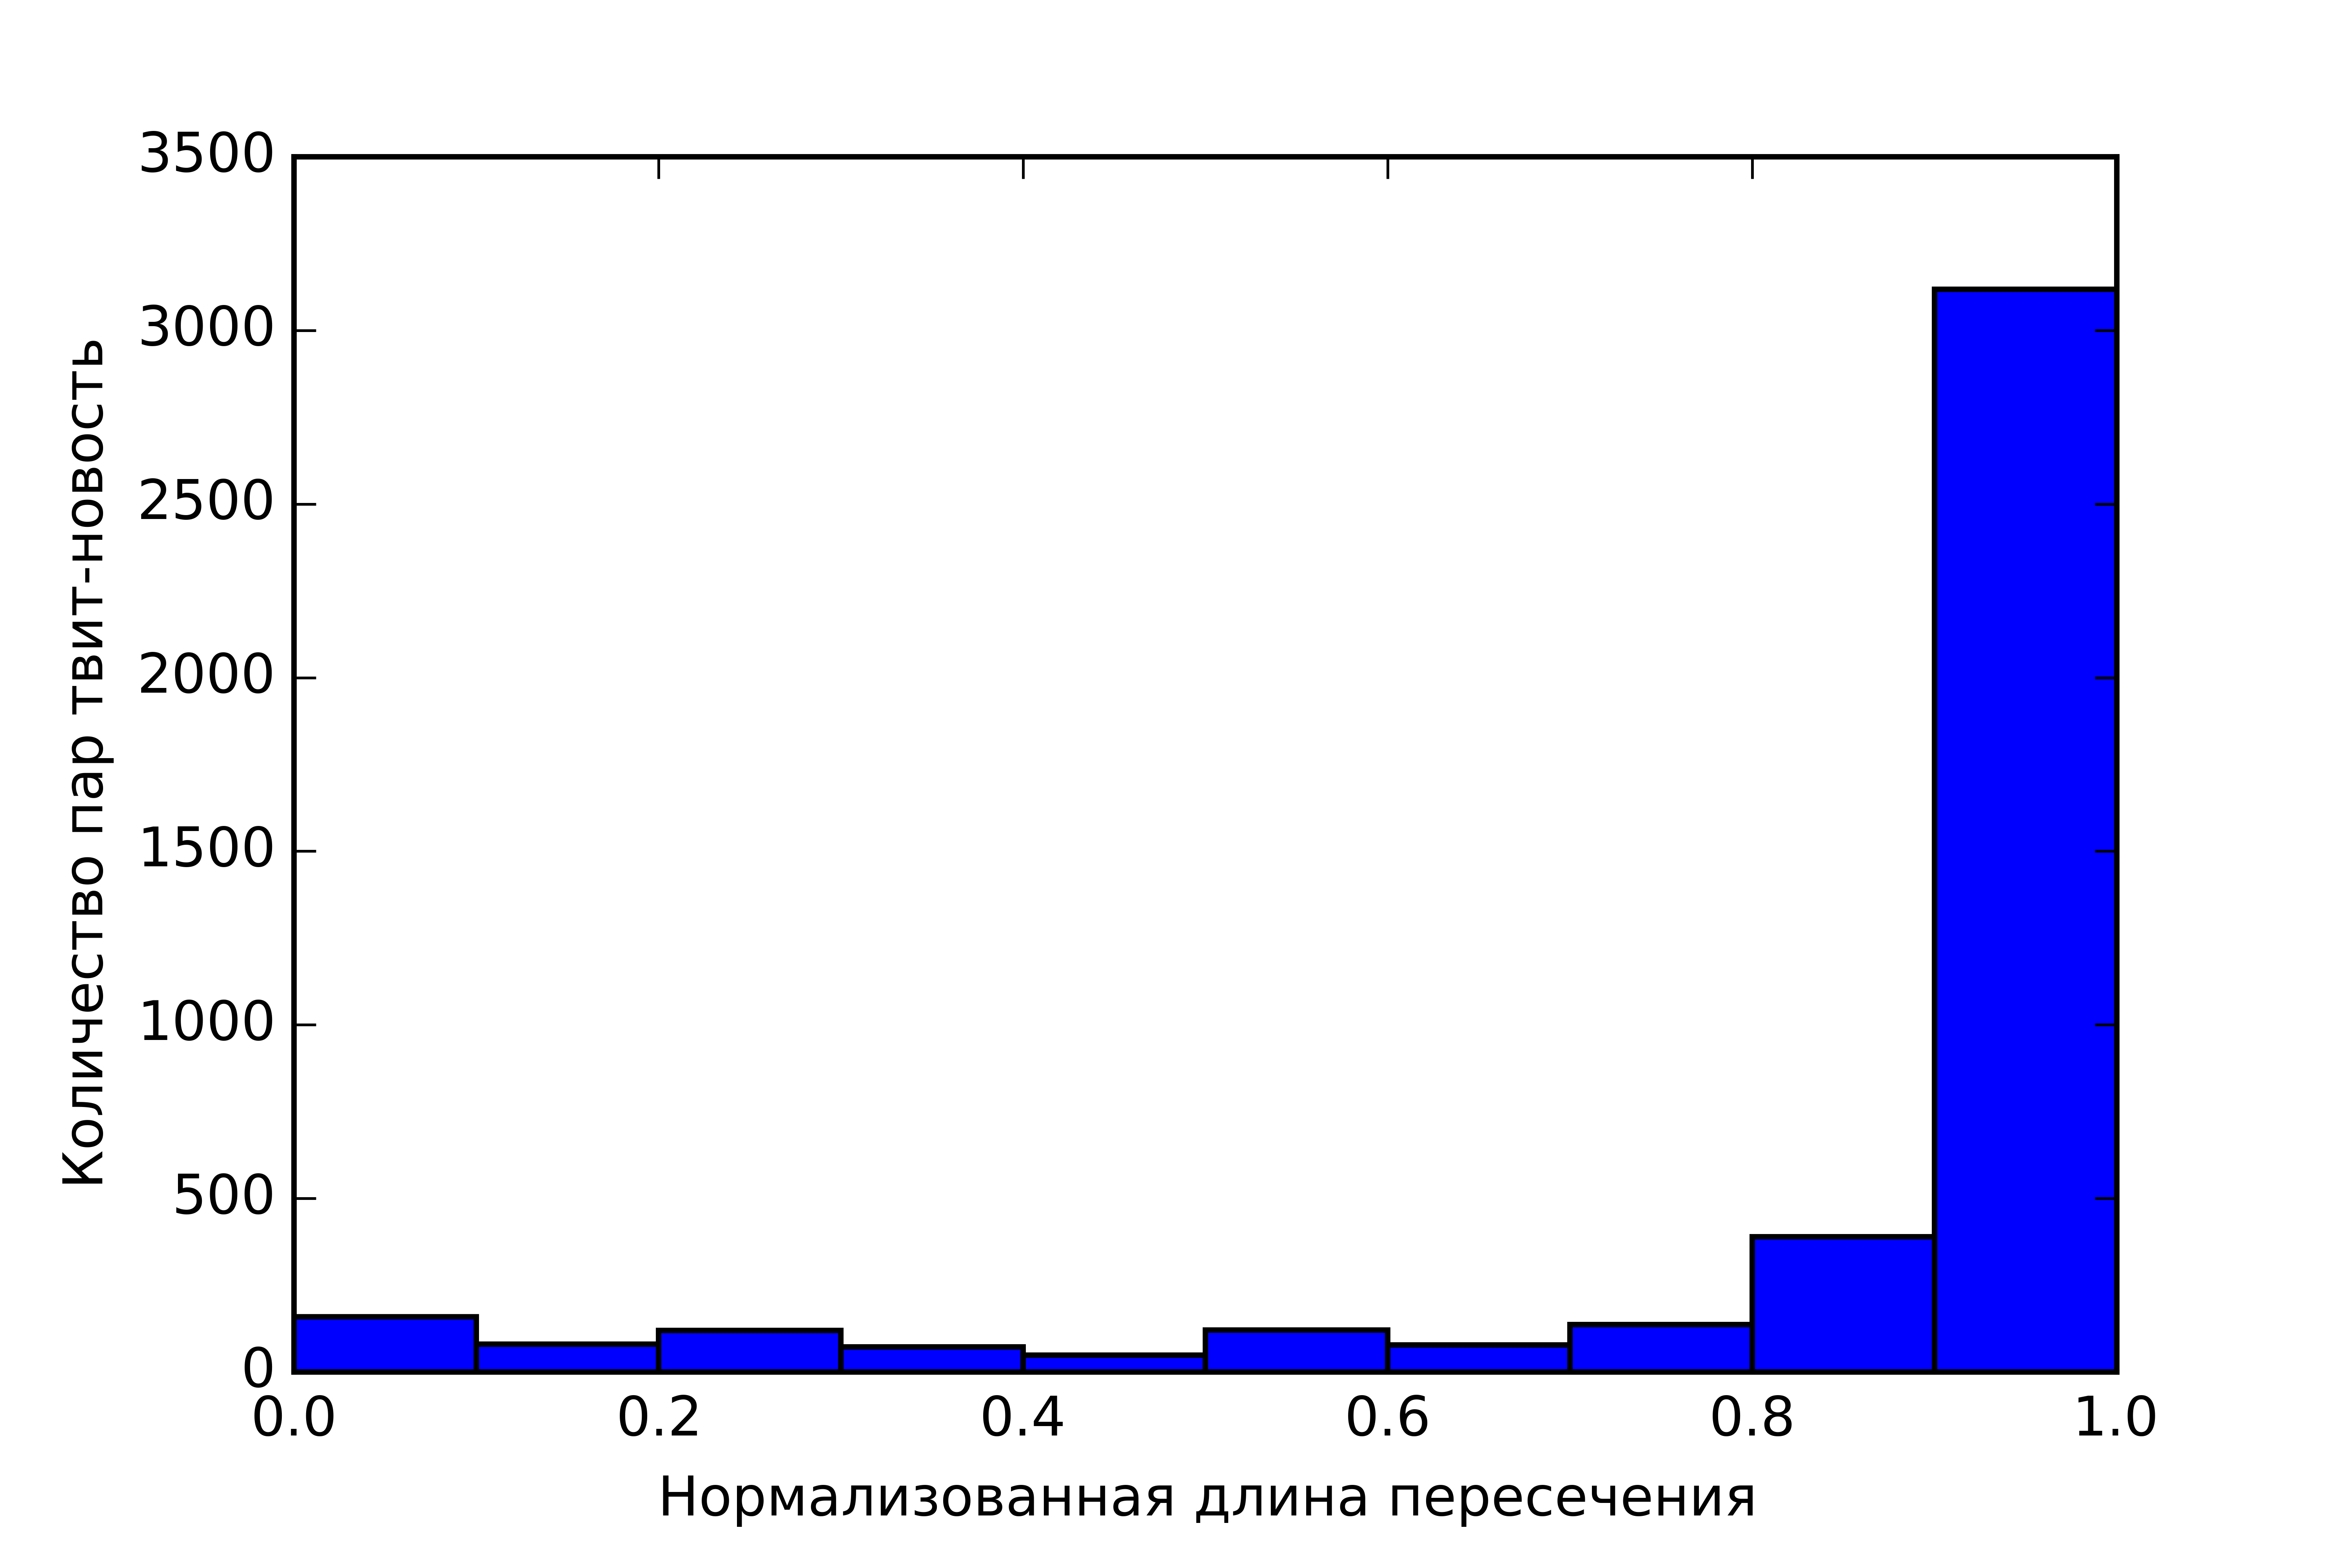
\includegraphics[scale=0.85]{dataset_auto_normalized_intersect_histogram.png}
            \caption{Зависимость количества пар твит-новости от нормализованный длины пересечения множества слов (автоматически размеченный набор данных).}
            \label{pic:auto_histogram}
        \end{figure}
        Как видно из рисунка~\ref{pic:auto_histogram} слова в подавляющем большинстве твитов полностью совпадают со словами в соответствующей новости.
        Среди 4324 пар твит-новость в 3082 парах твит полностью совпадает с заголовком новости. Остаётся 1242 пар, которые не являются просто копией заголовка, среди этих пар
        нас интересуют те, в которых твит не является обрезанной частью заголовка статьи.

        Для выявления количества пар, где твит содержит информацию не содержащуюся в заголовке статьи посмотрим на зависимость количества пар твит-новость от процента уникальных слов в твите,
        эта зависимость изображена на рисунке~\ref{pic:auto_percent}.
        \begin{figure}[h!]
            \center
            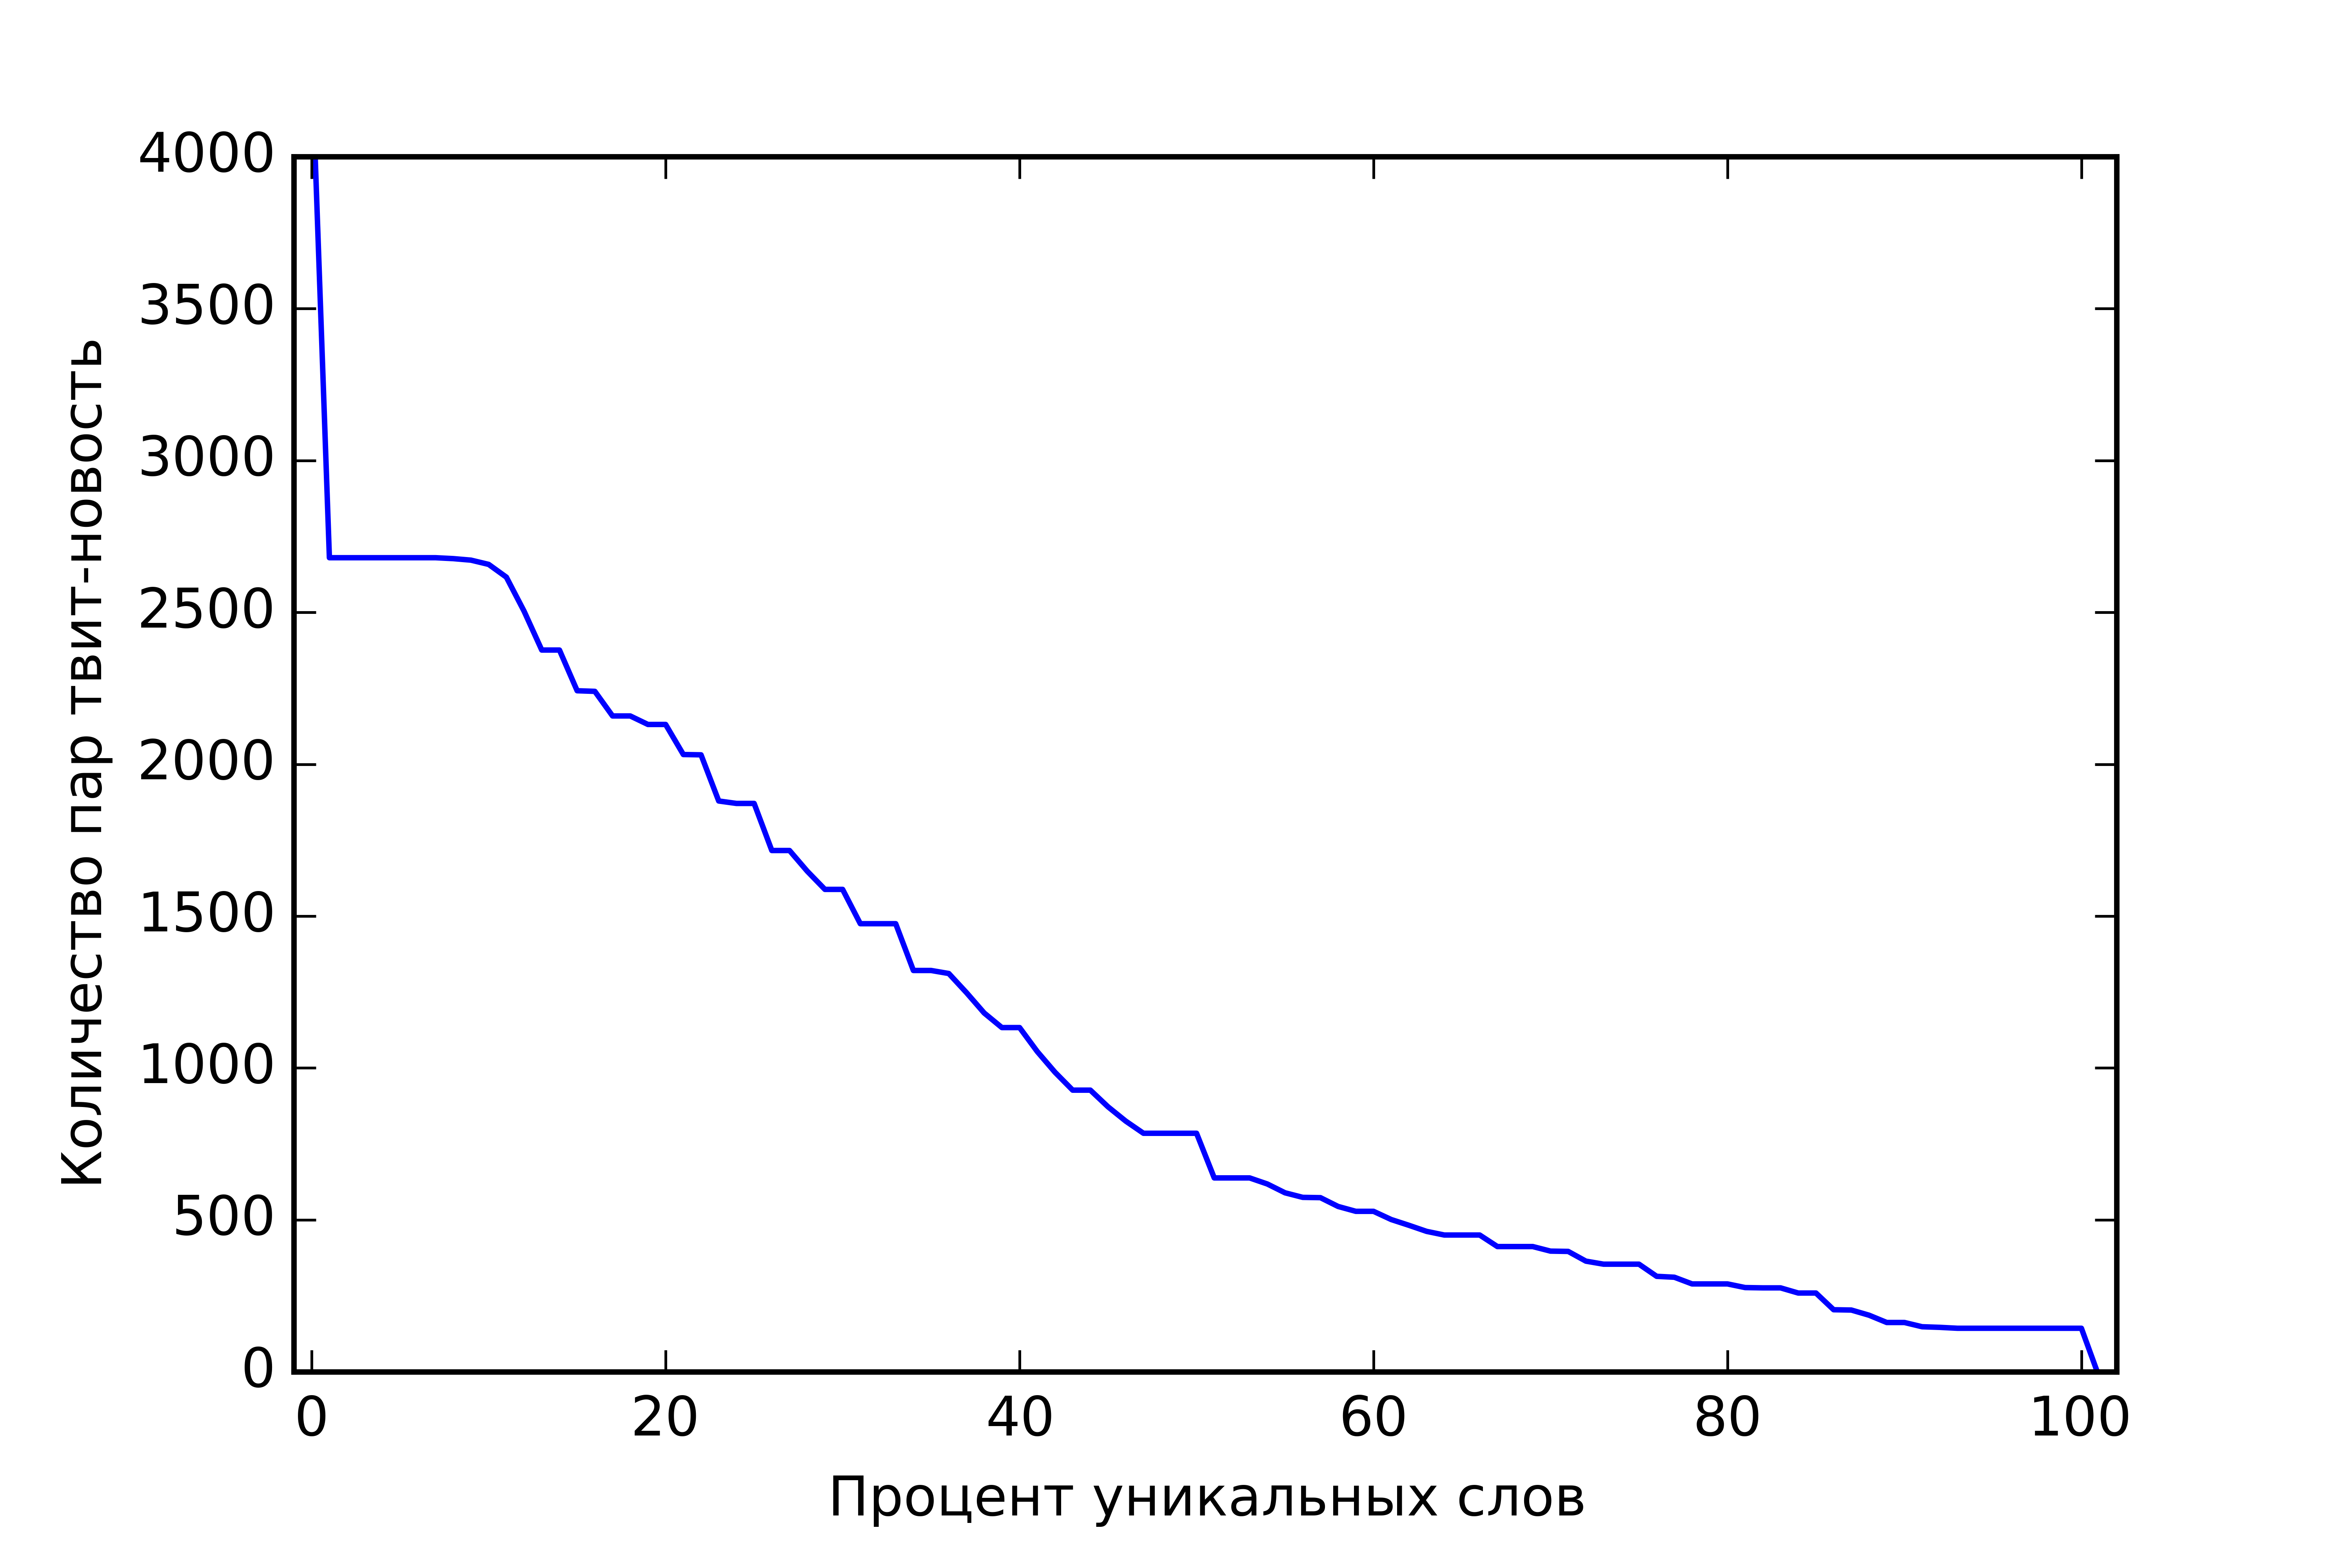
\includegraphics[scale=0.85]{dataset_auto_unique_words_percent.png}
            \caption{Зависимость количества пар твит-новости от процента уникальных слов в твите (автоматически размеченный набор данных).}
            \label{pic:auto_percent}
        \end{figure}
        Как видно из рисунка~\ref{pic:auto_percent} количество твитов более с чем половиной уникальных слов достаточно мало.

        На основе исследования зависимости можно получить грубую оценку количества нетривиальных связей.
        В исследуемом наборе данных таких связей порядка 500-1000, что очень мало и составляет примерно 12-23\% от общего числа пар.

    \subsubsection{Ручная разметка набор данных}
        Для получения большего количества нетривиальных пар твит-новость была предпринята ручная разметка набора данных.
        Для ручной разметки необходимо предподготовить данные. Основные этапы предподготовки данных:
        \begin{enumerate}
            \item на основе множества новостей строится список именованных сущностей $L$;
            \item случайным образом берётся подмножество $T$ множества твитов;
            \item из полученного множества $T$ удаляются все твиты, которые удолетворяют следующим правилам:
            \begin{enumerate}
                \item твит является ретвитом,
                \item твит содержит ссылку на URL с плохим доменным именем (под \textit{плохим} доменным именем подразумевается доменное имя,
                которое достаточно популярно и не ведёт на новостной источник, в работе использовался следующий список плохих доменных имён:\
                \url{apps.facebook.com}, \url{ask.fm}, \url{twitter.com}, \url{apps.facebook.com}, \url{www.instagram.com}, \url{vk.cc}),
                \item в приведённом к нормальной форме~(определение нормальной формы находится в главе\ref{subsubsec:lemma}) тексте твита содержится менее 2 слов из списка именованных сущностей $L$;
            \end{enumerate}
            \item c помощью метода определения схожести текстов на основе частотности употребления слов каждому твиту сопоставляется 10 наиболее схожих с ним новостей.
        \end{enumerate}
        В качестве результата предподготовки получается множества пар твит-ранжированный список новостей.

        Предподготовленные данные размечаются экспертом.
        Разметка заключается в записи специальной отметки рядом с подходящей новости из предложенного списка для каждого твита.
        Для каждого твита отмечается только одна, наиболее подходящая новость, или не отмечается ни одной.

        Было сформировано множество из 7373 пар твит-ранжированный список новостей. В нём экспертом было выявлено 1600 связей твит-новость.
        Получаем набор данных, состоящий из 1600 твитов, 13711 новостей, а также 1600 связей между ними.

        Для сравнения вручную построеннго набора данных с набором данных, полученным автоматически были построены две зависимости~---~
        зависимость количества пар твит-новость от длины пересечения слов твита и слов новости и  зависимость количества пар твит-новости от процента уникальных слов в твите.
        На рисунке~\ref{pic:manual_histogram} изображена зависимость количества пар твит-новость от длины пересечения слов твита и слов новости, нормализованная по длине новости.
        \begin{figure}[h!]
            \center
            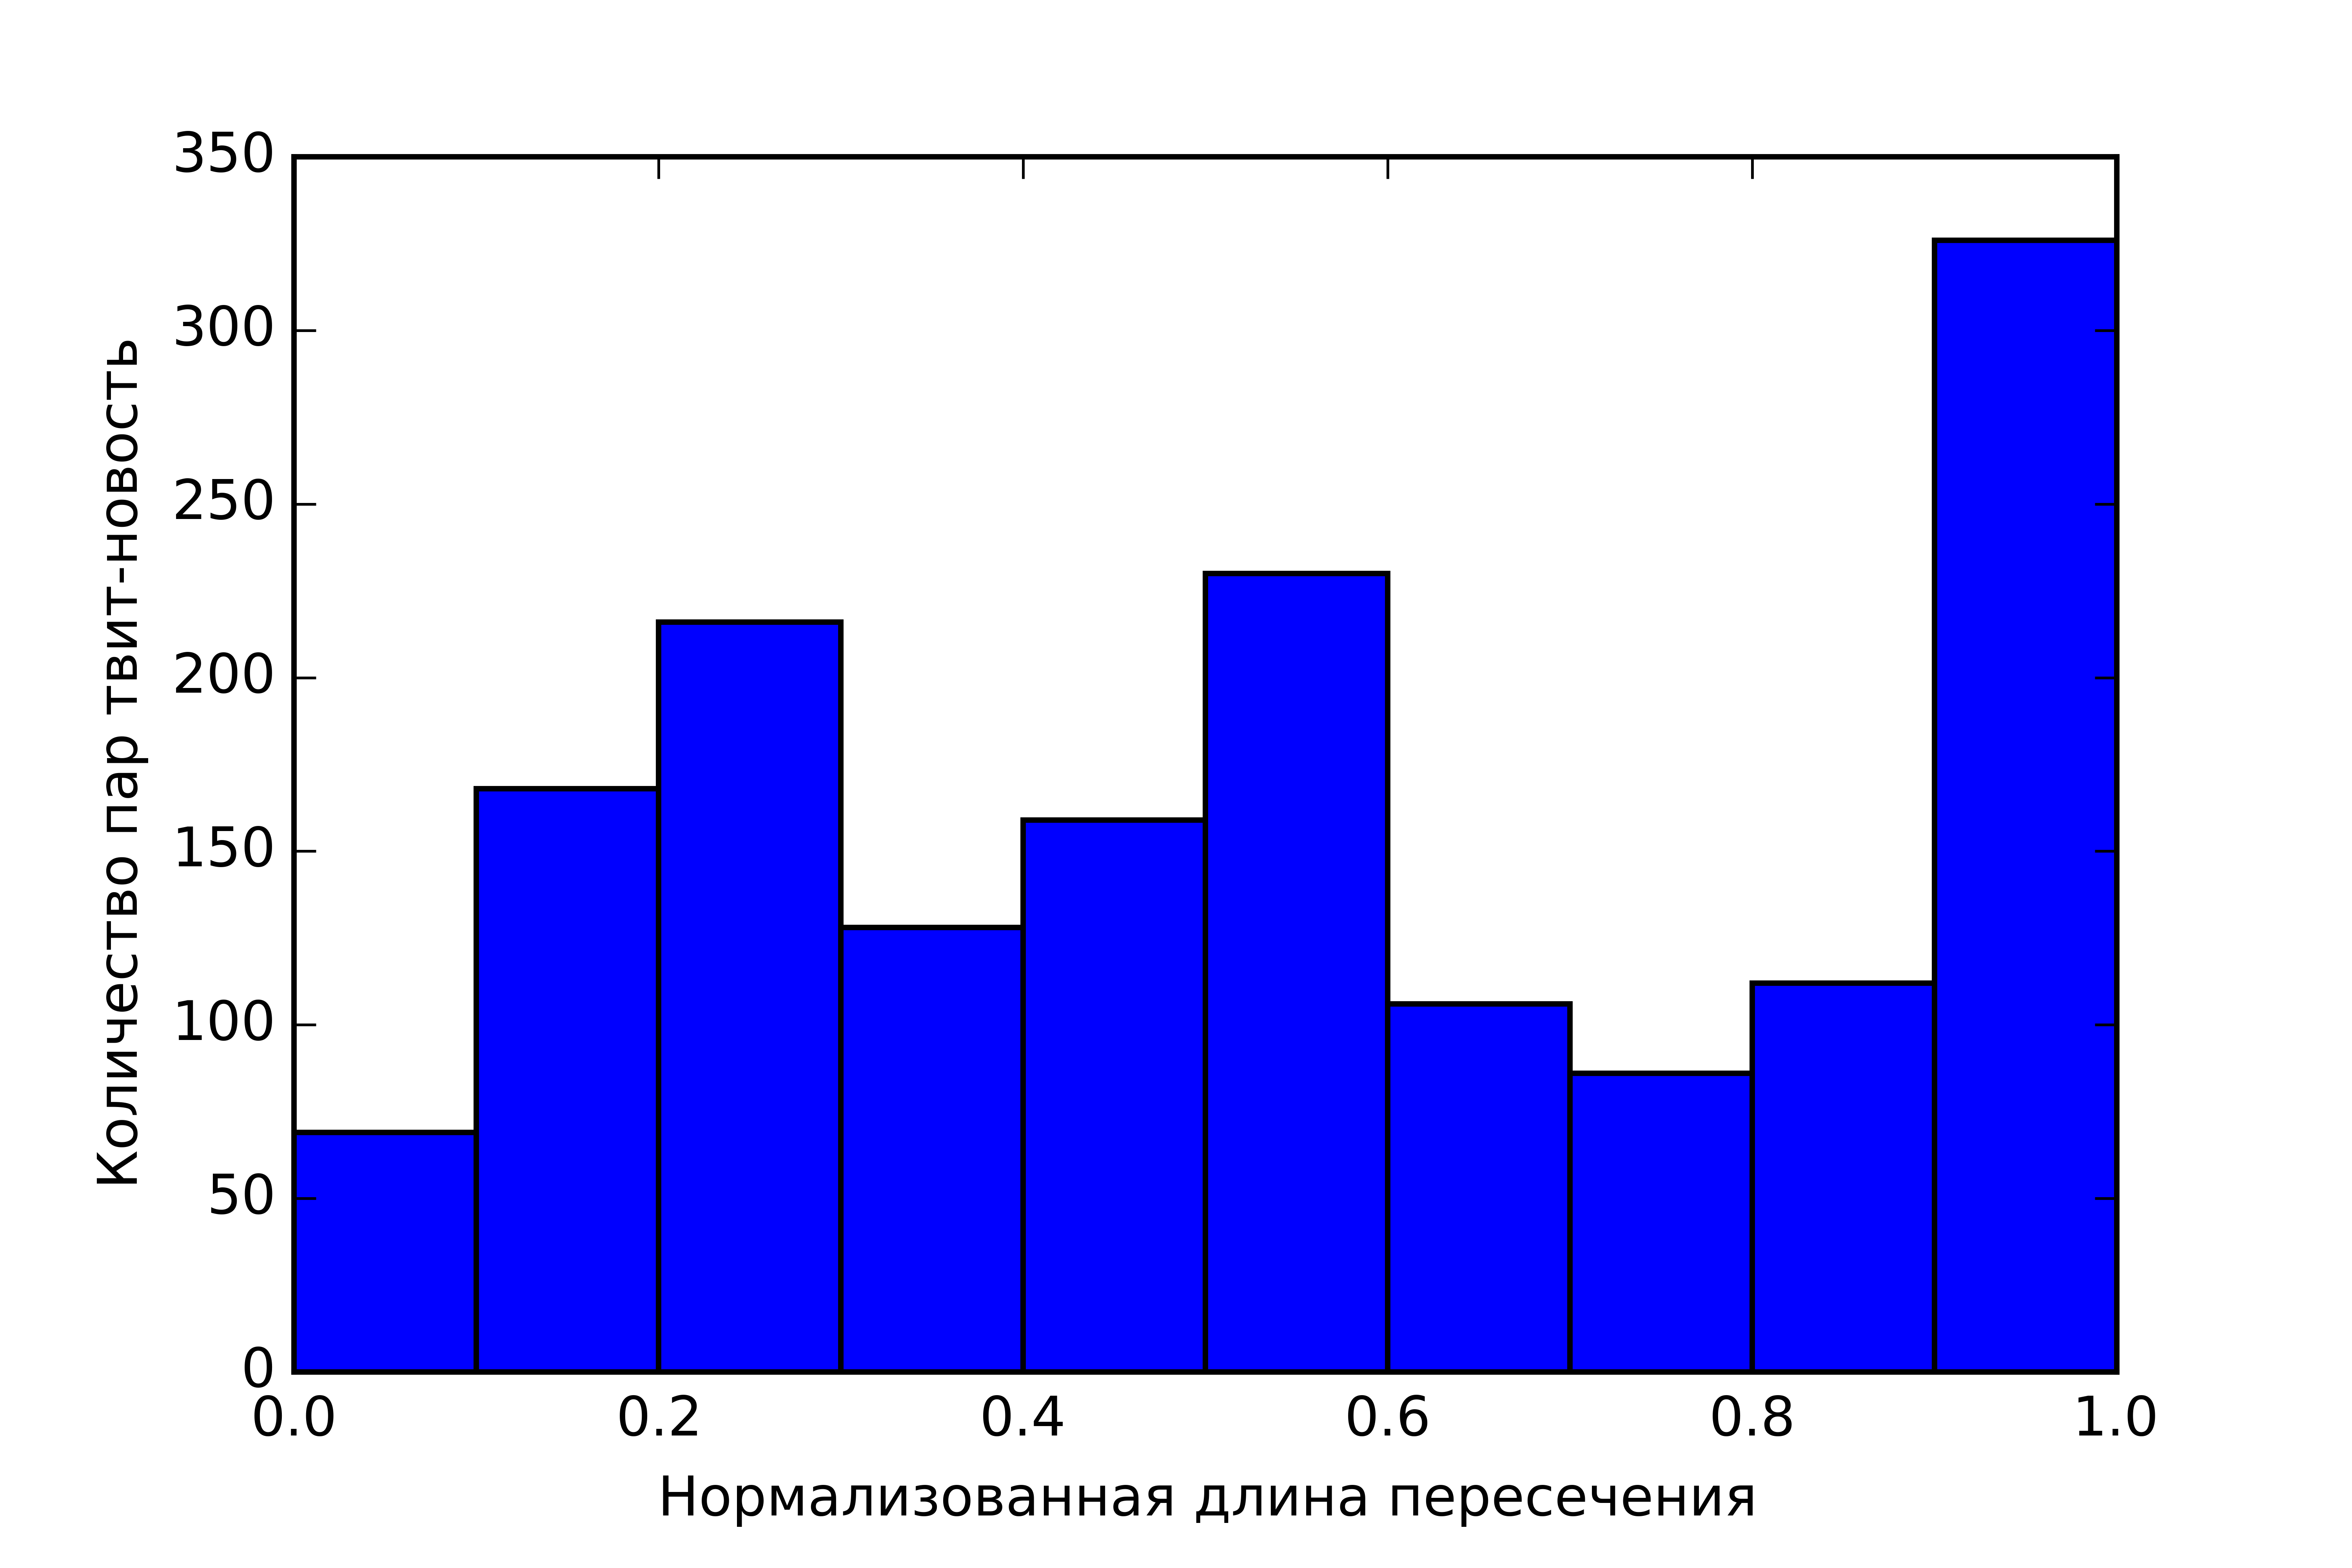
\includegraphics[scale=0.85]{dataset_manual_normalized_intersect_histogram.png}
            \caption{Зависимость количества пар твит-новости от нормализованный длины пересечения множества слов (вручную размеченный набор данных).}
            \label{pic:manual_histogram}
        \end{figure}
        Как видно из рисунка~\ref{pic:manual_histogram} было получено распределение намного более близкое к равномерному, чем в случае автоматически размеченного набора данных.

        На рисунке~\ref{pic:manual_percent} изображена зависимость количества пар твит-новость от процента уникальных слов в твите.
        \begin{figure}[h!]
            \center
            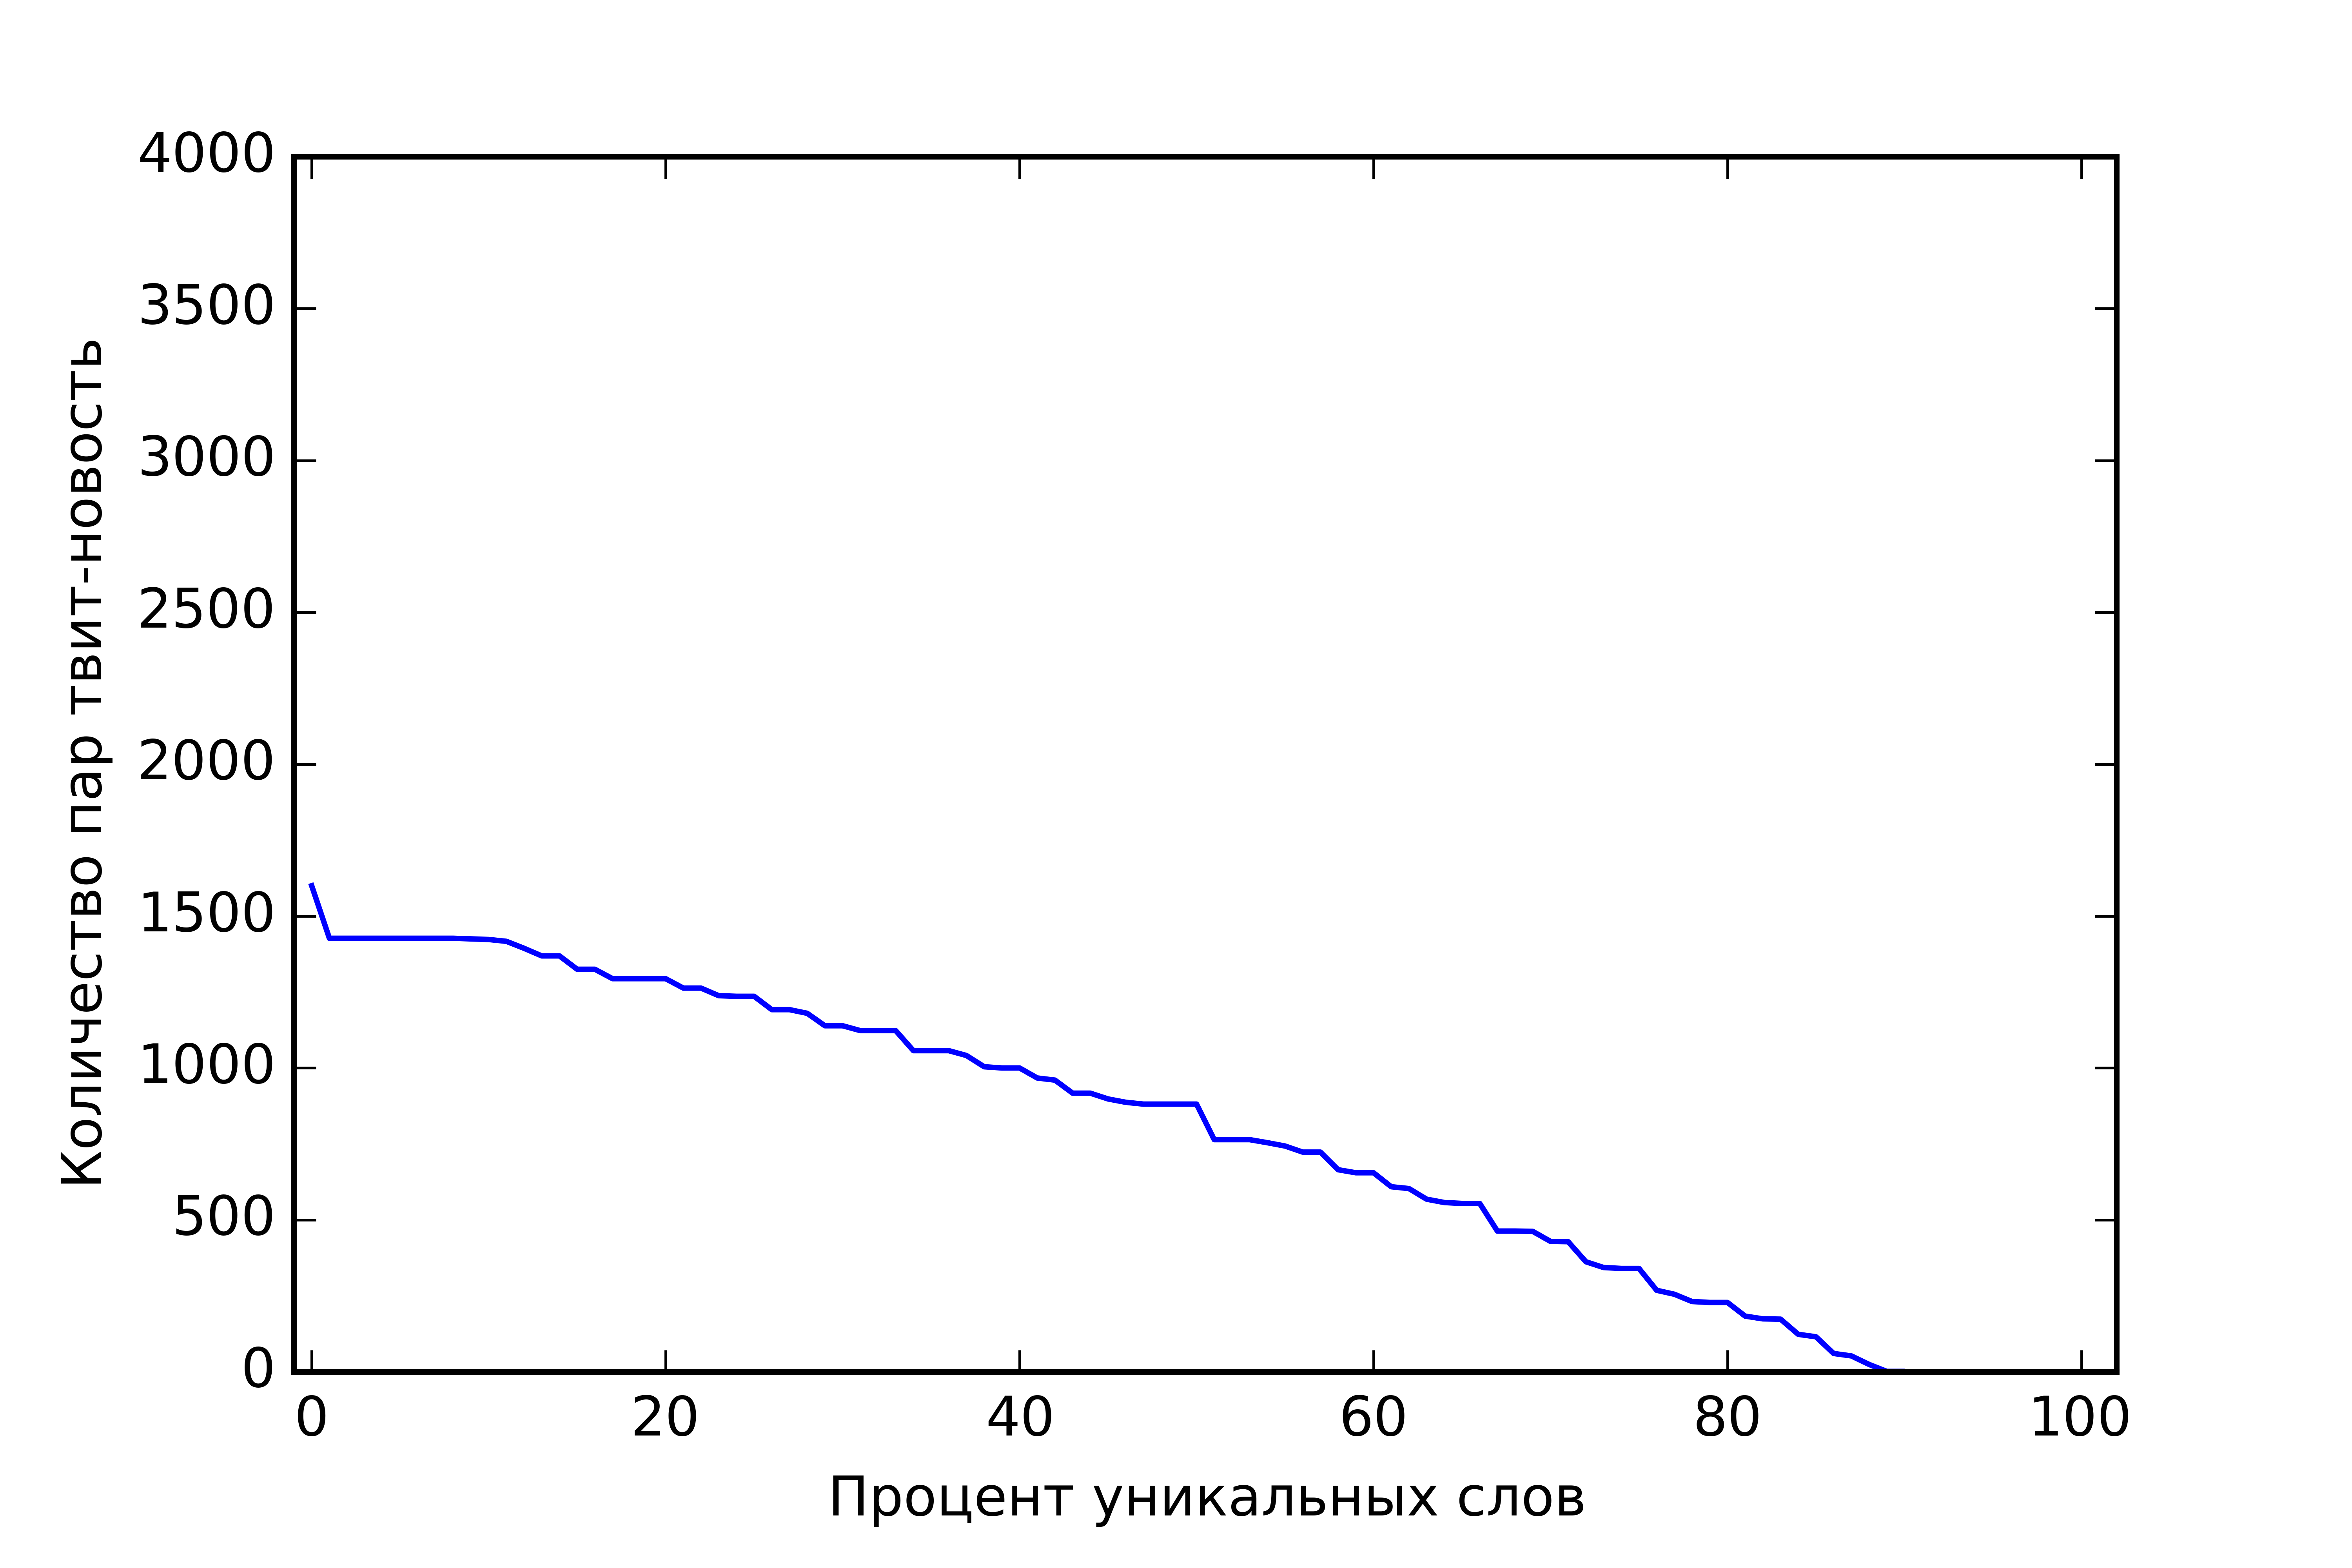
\includegraphics[scale=0.85]{dataset_manual_unique_words_percent.png}
            \caption{Зависимость количества пар твит-новости от процента уникальных слов в твите (вручную размеченный набор данных).}
            \label{pic:manual_percent}
        \end{figure}
        Как видно из рисунка~\ref{pic:manual_percent} количество твитов более с чем половиной уникальных слов сравнимо с аналогическим количеством в автоматически размеченном наборе данных,
        несмотря на то, что автоматически размеченный набор данных почти в три раза больше, чем вручную размеченный набор данных.

        Количественные значение полученных метрик приведены в таблице~\ref{tabular:dataset_stat}.
        \begin{table}[ht!]
            %\small
            \caption{Сравнение количества твитов \bigskip}
            \centering

            \label{tabular:dataset_stat}
            \begin{tabular}{|p{5cm}|c|c|}
                \hline
                \bf{\specialcell{Метрика}} &
                \bf{\specialcell{Автоматически размеченный \\ набор данных}} &
                \bf{\specialcell{Вручную размеченный \\ набор данных}} \\ \hline

                Количество связей & 4324 & 1600 \\ \hline
                Количество нетривиальных связей & 746 & 976 \\ \hline
                Процент нетривиальных связей от общего числа связей~(\%) & 17.25  & 61.00 \\ \hline
            \end{tabular}
        \end{table}
        Как видно из таблицы \ref{tabular:dataset_stat} вручную собранный набор данных намного более качественный, чем автоматический.
        Но как в ручном, так и в автоматическом наборе данных содержится очень мало нетривиальных связей твит-новость (в сравнении с количеством новостей).

    \subsubsection{Построение связей текст-текст}
        Реализация построения связей, описанного в главе \ref{subsubsec:linking}, привела к получению избыточного количества ложных связей на используемом наборе данных.
        По этой причине реализация была дополнена следующими эвристическими ограниченями:
        \begin{enumerate}
            \item удаление слишком популярных хэштегов~(слишком популярным считаем хэштег, который встретился более чем в 10 твитах из обучающей выборки);
            \item твиты, считаются связанными когда оба содержать не менее 2 одинаковых хэштегов или именованных сущностей;
            \item связь не устанавливается если тексты слишком похожи (если косинусная мера близости текстов больше 0.99);
            \item в случае установления связей на основе времени публикации и схожести текстов, слишком не похожие тексты отбрасываются
            (слишком не похожие тексты это тексты с мерой близости меньше чем 0.3).
        \end{enumerate}

    \subsubsection{Сформированные набор данных}
        На основе собранной информации было сформировано несколько базовых эталонных наборов, а именно:
        \begin{enumerate}
            \item auto~---~автоматически размеченный набор данных;
            \item manual~--~вручную размеченный набор данных;
            \item total~---~набор данных состоящий из объединения всех размеченных связей (то есть объединение auto и manual);
            \item cutted~---~набор данных, основанный на наборе total, в котором количество новостей сравнимо с количеством твитов~
            (набор данных создавался для изучения влияния соотношения количества новостей и твитов на качество установления связей).
        \end{enumerate}
        Также рассматриваются эталонные наборы данных без тривиальных связей, подобный набор образуется путём удаления из базового эталонного набора твитов, создающих тривиальную связь.
        Обозначим эталонные наборы данных с удалёнными тривиальными связями как auto\_nt, manual\_nt, total\_nt и cutted\_nt,
        полученные путём удаления тривиальных связей из базовых эталонных наборов auto, manual, total и cutted, соответственно.

        Ключевая информация характеризующая эталонные наборы представлена в таблице~\ref{tabular:dataset_info}.
        \begin{table}[ht!]
            %\small
            \caption{Сводная таблица по эталонным наборам данных\bigskip}
            \centering

            \label{tabular:dataset_info}
            \begin{tabular}{|c|c|c|}
                \hline
                \bf{\specialcell{Набор данных}} &
                \bf{\specialcell{Количество твитов}} &
                \bf{\specialcell{Количество новостей}} \\ \hline
                manual & 1600 & 13711 \\ \hline
                auto & 4324 & 13711 \\ \hline
                total & 5798 & 13711 \\ \hline
                cutted & 5798 & 6011 \\ \hline
                manual\_nt & 976 & 13711 \\ \hline
                auto\_nt & 746 & 13711 \\ \hline
                total\_nt & 1709 & 13711 \\ \hline
                cutted\_nt & 1709 & 6011 \\ \hline
            \end{tabular}
        \end{table}


    \subsection{Метод WTMF}
    Модель для метода WTMF построена на основе мнзаранее подготовленного набора данных.
    В контексте работы набор данных состоит из множества новостей и твитов, из которых в процессе работы извлекается набор текстов
    ~(для твита~---~текст твита, для новости~---~конкатенация заголовка и краткого изложения статьи).

    По множеству текстов, которые получены из набора данных, построена модель, пригодная для сериализации, состоящая из матрицы $P$
    ~(здесь и далее используются обозначения введённые в главе \ref{subsubsec:wtmf}).
    Построение модели зависит от четырёх констант:
    \begin{enumerate}
        \item $K$~---~размерность вектора, по которому производится сравнение~
        (если TF-IDF матрица $X$ была размера $M \times N$, то по завершении работы алгоритма будут получены две матрицы $P$ размера $K \times M$ и $Q$ размера $K \times N$);
        \item $I$~---~число итераций алгоритма построения модели;
        \item $w_M$~---~коэффициент, задающий вес негативного сигнала при построении матрицы весов $W$;
        \item $\lambda$~---~регуляризирующий член.
    \end{enumerate}

    Применение полученной модели на множество твитов представляет собой следующий процесс:
    сначала строится TF-IDF матрица $X$ для новостей из набора данных и множества твитов, затем на основе новой матрицы $X$ строится весовая матрица $W$,
    и наконец на основе построенных матриц $X$ и $W$ и посчитанной на этапе обучения матрицы $P$ выполняется половина итерации алгоритма обучения,
    а именно получение матрицы $Q$ по матрице $P$:
    $$Q_{\cdot, j} = (P W'_j P^T + \lambda I)^{-1} P W'_j X_{j,\cdot}.$$
    В результате получаем вектора для сравнения твитов из заданного множества.
    \subsection{Метод WTMF-G}
    Построение модели для метода WTMF-G основывается на построение модели метода WTMF.
    Набор данных состоит из множества новостей и твитов и связей вида текст-текст, из которых, в процессе работы извлекается набор текстов.
    ~(для твита~---~текст твита, для новости~---~конкатенация заголовка и краткого изложения статьи).

    По множеству текстов, которые получены из набора данных, построена пригодная для сериализации модель, представляющая собой матрицу $P$.
    Построение модели зависит от четырёх констант:
    \begin{enumerate}
        \item $K$~---~размерность вектора, по которому производится сравнение~
        (если TF-IDF матрица $X$ была размера $M \times N$, то по завершении работы алгоритма будут получены две матрицы $P$ размера $K \times M$ и $Q$ размера $K \times N$);
        \item $I$~---~число итераций алгоритма построения модели;
        \item $w_M$~---~коэффициент, задающий вес негативного сигнала при построении матрицы весов $W$;
        \item $\delta$~---~коэффициент, задающий степень влияния связей вида текст-текст.
    \end{enumerate}

    Применение полученной модели на множество твитов производится аналогично применению модели для метода WTMF за исключением двух моментов:
    во-первых, необходимо на основе новостей из набора данных и множества твитов перестроить связи текст-текст, во-вторых получение матрицы $Q$ происходит по следующей формуле:
    $$Q_{\cdot, j} = (P W'_j P^T + \lambda I + \delta  L_j^2 Q_{\cdot,n(j)} diag(L^2_{n(j)})Q_{\cdot,n(j)}^T)^{-1}   (P W'_j X_{j,\cdot} + \delta  L_j Q_{\cdot,n(j)} L_{n(j)}).$$
    В результате получаем вектора для сравнения твитов из заданного множества.
    
\subsection{Эффективная работа с матрицами}
    Построение и применение моделей WTMF и WTMF-G требует большого количества операций над матрицами, что на практике занимает продолжительное время.
    Поэтому задача по повышению эффективности работы с матрицами актуальна.

    Для эффективной работы с матрицами используются программные библиотеки для языка Python numpy и
    scipy~(базируется на библиотеке numpy и расширяет её функционал).

    Оптимизируется формула получения строк матрицы $P$, используемая при построении моделей WTMF и WTMF-G.
    На каждой итерации построения модели происходит многократное выполнение формулы (количество выполнений порядка $10^4$, зависит от размера корпуса):
    $$P_{i, \cdot} = (Q W'_i Q^T + \lambda I)^{-1} Q W'_i X_{i,\cdot}^T.$$

    В начале была написана наивная реализация алгоритма, которая показала производительность, не приемлемую в рамках решения задачи.
    Затем наивная реализация оптимизировалась следующим образом:
    \begin{enumerate}
        \item переход к перемножению матриц с использованием высокопроизводительной библиотеки для языка С OpenBlass~(в библиотеке numpy существует возможность перейти к использованию для работы с матрицами некоторых библиотек, написанных на языке С~\cite{blas_installation});
        \item сохранение в отдельной переменной переиспользуемых результатов вычислений над матрицами;
        \item переписывание кода для работы с разреженными матрицами;
        \item удаление лишних приведений матриц к формату python list и обратно.
    \end{enumerate}
    Результаты оптимизации приведены в таблице~\ref{tabular:matrix_optimization}.

    \begin{table}[ht!]
        %\small
        \caption{Оптимизация работы с матрицами\bigskip}
        \centering

        \label{tabular:matrix_optimization}
        \begin{tabular}{|p{5cm}|c|c|}
            \hline
            \bf{\specialcell{Добавленная \\ оптимизация}} &
            \bf{\specialcell{Время за \\ 100 итераций~(c)}} &
            \bf{\specialcell{Прирост \\ производительности \\ (раз) }} \\ \hline

            Наивная реализация & 205 & 1 \\ \hline
            Перемножение с помощью OpenBlass & 55 & 3.73 \\ \hline
            Переиспользование результатов & 15.15 & 3.63 \\ \hline
            Работа с разреженными матрицами & 0.75 & 20.2 \\ \hline
            Сокращение количества приведений типов & 0.63 & 1.21 \\ \hline
        \end{tabular}
    \end{table}
    Получили, что оптимизированное решение работает в 325 раз быстрее наивной реализации.
    Дальнейшая оптимизация не производилась, так как получено решение работающее за приемлемое время.
%    Дополнительную оптимизацию можно произвести с помощью использования библиотек для работы с матрицами, использующих видеокарт
%
%
%
%    идеи по дальнейшей оптимизации: CUDA

